% !TeX program = xelatex
% 编译：xelatex 13-典型信号的傅里叶变换.tex（VS Code 的 LaTeX Workshop 会读上一行，自动用 xelatex）
% 来源：2022 浙江大学《信号与系统》胡浩基老师，傅里叶与伽罗华、傅里叶变换的定义、典型信号的傅里叶变换。教材 3.2.3 节（第 97～99 页，式 3-51、3-53）；u(t) 的傅里叶变换在第 107 页式 3-83。
% 体例：历史 → 从傅里叶级数推出傅里叶变换 → 定义 → 正变换推反变换的证明 → 七个典型傅里叶变换对（每个：推导 → 图 → 例题）。
% 公式编号按课上最终的用法：⑥ 是 u(t)，⑦ 是 cos 与 sin（两者合成一条）。
% 图中曲线用 TikZ 直接按公式计算；例题数值按板书核对过。
\documentclass[UTF8,a4paper,11pt]{ctexart}
\usepackage{amsmath,amssymb}
\usepackage{geometry}
\geometry{margin=2.4cm}
\usepackage{xcolor}
\usepackage{mdframed}
\usepackage{booktabs}
\usepackage{needspace}
\usepackage{array}
\usepackage{enumitem}
\usepackage{tikz}
\usetikzlibrary{arrows.meta,positioning,calc,patterns}
\usepackage{float}
\usepackage{fancyhdr}
% 页眉页脚清空，只在右下角保留页号（含首页）
\fancypagestyle{plain}{%
  \fancyhf{}%
  \fancyfoot[R]{\thepage}%
  \renewcommand{\headrulewidth}{0pt}%
  \renewcommand{\footrulewidth}{0pt}}
\usepackage[hidelinks,unicode,bookmarksnumbered,bookmarksopen=true,bookmarksopenlevel=2,pdftitle={典型信号的傅里叶变换}]{hyperref}
\usepackage{bookmark}% XeTeX 下 hyperref 自带的大纲不生效，用 bookmark 宏包生成 PDF 书签（需编译两遍）

\setCJKmainfont{Songti SC}[BoldFont={Songti SC Bold}]
\setCJKsansfont{PingFang SC}

\newcommand{\Sa}{\operatorname{Sa}}
\newcommand{\dd}{\mathrm{d}}
\newcommand{\F}{\mathcal{F}}

\newmdenv[backgroundcolor=blue!4,linecolor=blue!50!black,linewidth=1pt,innertopmargin=6pt,innerbottommargin=6pt]{rememberbox}
\newenvironment{remember}{\begin{rememberbox}\textbf{重点}\par\smallskip}{\end{rememberbox}}
\newmdenv[backgroundcolor=yellow!8,linecolor=orange!70!black,linewidth=1pt,innertopmargin=6pt,innerbottommargin=6pt]{notebox}
\newenvironment{note}{\begin{notebox}\textbf{说明}\par\smallskip}{\end{notebox}}

% ---------------------------------------------------------------- 画图用的小宏
% 坐标轴：\taxes[自变量名]{横轴起点}{横轴终点}{纵轴顶端}{纵轴底端}。原点标 0（放在左下，避开纵轴）。
\newcommand{\taxes}[5][t]{%
  \draw[->] (#2,0) -- (#3,0) node[right,font=\scriptsize] {$#1$};
  \draw[->] (0,#5) -- (0,#4);
  \node[anchor=north east,font=\tiny,gray!60!black,inner sep=1pt] at (0,-0.02) {$0$};}
% 横轴刻度 \xt{位置}{标签}（标在轴下方）、\xtu{位置}{标签}（标在轴上方）、纵轴刻度 \yt{位置}{标签}：刻度线 + 白底数字。
\newcommand{\xt}[2]{\draw (#1,0) -- (#1,-0.1) node[anchor=north,font=\tiny,gray!60!black,fill=white,inner sep=0.6pt] {$#2$};}
\newcommand{\xtu}[2]{\draw (#1,0) -- (#1,0.1) node[anchor=south,font=\tiny,gray!60!black,fill=white,inner sep=0.6pt] {$#2$};}
\newcommand{\yt}[2]{\draw (0,#1) -- (-0.1,#1) node[anchor=east,font=\tiny,gray!60!black,fill=white,inner sep=0.6pt] {$#2$};}
% 横轴刻度，标签放到曲线下方：\xtl{位置}{标签}{标签所在的纵坐标}，中间用细点线连到刻度。
\newcommand{\xtl}[3]{\draw (#1,0) -- (#1,-0.08); \draw[gray!55,densely dotted] (#1,-0.08) -- (#1,#3);
  \node[anchor=north,font=\tiny,gray!60!black,fill=white,inner sep=0.6pt] at (#1,#3) {$#2$};}
\tikzset{every picture/.style={baseline=(current bounding box.center)}}% 并排的图与中间的箭头按中线对齐
\tikzset{>=stealth,
  sig/.style={thick,blue!60!black},
  res/.style={thick,red!70!black},
  grn/.style={thick,green!45!black},
  imp/.style={very thick,->,>={Stealth[length=5pt]}}}

% ---------------------------------------------------------------- 标题层级
\definecolor{secblue}{RGB}{31,78,121}
\definecolor{exorange}{RGB}{190,90,10}
\definecolor{ptteal}{RGB}{0,110,110}
\ctexset{
  section={format=\raggedright\Large\bfseries\color{secblue},
           beforeskip=3.2ex plus 1ex minus .5ex, afterskip=1.4ex,
           aftertitle={\par\nobreak\vspace{-1.1ex}\noindent\textcolor{secblue}{\rule{\linewidth}{0.8pt}}\par\nobreak\vspace{0.6ex}}},
  subsection={format=\raggedright\large\bfseries\color{secblue},
              beforeskip=2.4ex plus .8ex minus .4ex, afterskip=1.0ex}
}
% 例题标题：\example{标题}{结论}{附注}，附注一般留空。
\newcounter{ex}[section]
\newcommand{\example}[3]{%
  \refstepcounter{ex}\phantomsection
  \addcontentsline{toc}{subsubsection}{例 \theex\ #1（#2）}%
  \par\addvspace{1.6ex}\noindent
  {\setlength{\fboxsep}{3pt}%
   \colorbox{exorange}{\textcolor{white}{\textbf{例~\theex}}}\ %
   \textcolor{exorange}{\textbf{#1}}\ {\footnotesize\textcolor{gray!70!black}{#3}}%
   \hfill\colorbox{exorange!12}{\small\textcolor{exorange}{#2}}\par}%
  \nobreak\vskip0.6ex\relax\csname @afterheading\endcsname}
% 小标题（接着同一段往下写，不进大纲）：青色三角 + 粗体。
\newcommand{\point}[1]{\par\addvspace{1ex}\noindent\textcolor{ptteal}{$\blacktriangleright$\,\textbf{#1}}\ }

\title{典型信号的傅里叶变换\\\large 浙江大学 2022《信号与系统》（胡浩基）第三章听课笔记}
\author{}
\date{}

\begin{document}
\pagestyle{plain}
\maketitle

%==================================================================
\section{傅里叶与伽罗华}\label{sec:history}
第三章第一节讲完了傅里叶级数，第二节讲傅里叶变换。两节之间先看一段历史。

\point{傅里叶。}傅里叶(Joseph Fourier，1768--1830)在 1807 年提出用三角级数表示函数，最初不被承认。不被承认的时间并不长：几年后，大家发现用他的方法求解热传导方程很有应用价值（1811 年他以此参加法国科学院的有奖征文并获奖），他在科学界的地位由此确立，1817 年当选法国科学院院士。

\point{伽罗华。}1830 年，19 岁的伽罗华(Évariste Galois，1811--1832)把论文投给法国科学院，论文交到傅里叶手里；不久傅里叶去世，这篇论文被搁置并遗失。1831 年他再次投稿，审稿的泊松(Siméon Denis Poisson)认为难以看懂，把论文退了回来。论文的内容是：
\begin{itemize}[nosep]
\item 五次及五次以上的方程没有统一的求根公式（不能用根式求解）；
\item 还给出了这类方程在什么情况下有求根公式，是一个充要条件的证明；
\item 证明的整个流程开创了一个崭新的数学分支——\textbf{群论}(group theory)。
\end{itemize}
伽罗华的工作生前没有得到肯定。1832 年，20 岁的他因感情纠葛与情敌决斗，中枪身亡。

十几年后（1843 年），同在法国科学院工作的数学家刘维尔(Joseph Liouville)读到伽罗华留下的论文（每篇投稿都留有备份），用了三个多月研究，确认伽罗华已经把这个问题完全解决，并于 1846 年将其发表。

\point{那个年代的法国。}傅里叶的年代，法国在数学方面人才辈出。论文征集、审稿、院士等科研制度在那时建立完善，这些制度沿用至今。信号与系统的理论体系，大部分是法国人在 1800 年到 1900 年前后这一百年左右奠定的；1930--1940 年代，美国的工程界把它变成了目前的各种工程应用。

%==================================================================
\section{从傅里叶级数到傅里叶变换}\label{sec:derive}
\subsection{出发点：傅里叶级数只针对周期信号}
傅里叶级数的两个公式：
\[
x(t)=\sum_{k=-\infty}^{+\infty}a_k\,e^{jk\omega_0t},\qquad
a_k=\frac1{T_0}\int_{T_0}x(t)\,e^{-jk\omega_0t}\,\dd t ,
\]
使用时要知道两个条件：\textcircled{\scriptsize 1} $x(t)$ 以 $T_0$ 为周期；\textcircled{\scriptsize 2} $\omega_0=\frac{2\pi}{T_0}$。

傅里叶级数针对的是周期函数。下一步的核心目的是\textbf{把傅里叶级数推广到非周期函数上}。非周期函数就是在任何地方都没有周期；也可以把它理解为\textbf{周期 $T_0=+\infty$}。

\subsection{推导}
\point{第一步：定义一个函数。}定义
\[
X(j\omega)=\int_{T_0}x(t)\,e^{-j\omega t}\,\dd t .
\]
对照 $a_k$ 的公式：$a_k$ 里的积分正是把 $X(j\omega)$ 里的 $\omega$ 换成 $k\omega_0$，其他都不变，所以
\[
a_k=\frac1{T_0}\int_{T_0}x(t)\,e^{-jk\omega_0t}\,\dd t=\frac1{T_0}\,X(jk\omega_0).
\]

\point{$j$ 只是一个占位符。}$X(j\omega)$ 的自变量是 $\omega$，括号里的 $j$ 没有实际意义，写不写都一样，有的书直接写成 $X(\omega)$。多数信号与系统教材沿用奥本海姆(Oppenheim)的写法加上 $j$，是为了与第四章离散时间的傅里叶变换区分开。初学时容易在这里搞混。

\point{第二步：代回傅里叶级数。}把 $a_k$ 代入 $x(t)$ 的公式，再利用 $\omega_0=\frac{2\pi}{T_0}$：在求和号里乘一个 $\omega_0$，前面再除以一个 $\omega_0$，
\[
x(t)=\frac1{T_0}\sum_{k=-\infty}^{+\infty}X(jk\omega_0)\,e^{jk\omega_0t}
=\frac1{\omega_0T_0}\sum_{k=-\infty}^{+\infty}X(jk\omega_0)\,e^{jk\omega_0t}\cdot\omega_0
=\frac1{2\pi}\sum_{k=-\infty}^{+\infty}X(jk\omega_0)\,e^{jk\omega_0t}\cdot\omega_0 ,
\]
最后一步用了 $\omega_0T_0=2\pi$。

\point{第三步：令周期趋于无穷。}非周期的 $x(t)$ 可以理解为 $T_0=+\infty$，于是 $\omega_0=\frac{2\pi}{T_0}\to0$：
\[
\text{非周期 }x(t)\ \Longrightarrow\ T_0=+\infty\ \Longrightarrow\ \omega_0=\frac{2\pi}{T_0}\to0 .
\]
此时上面的求和就变成积分：
\[
x(t)=\frac1{2\pi}\int_{-\infty}^{+\infty}X(j\omega)\,e^{j\omega t}\,\dd\omega .
\]
这是黎曼积分(Riemann integral)定义的形式：把 $\omega$ 轴切成宽度为 $\omega_0$ 的小段，每一段取函数值 $X(jk\omega_0)e^{jk\omega_0t}$，乘以小段的宽度 $\omega_0$ 再相加；$\omega_0\to0$ 时，这个和就等于积分。

同时，$T_0\to+\infty$ 时，$X(j\omega)$ 定义中\textbf{一个周期上的积分也变成了 $(-\infty,+\infty)$ 上的积分}。这样就得到傅里叶变换的一对公式（第 \ref{sec:def} 节）。

\begin{figure}[H]
\centering
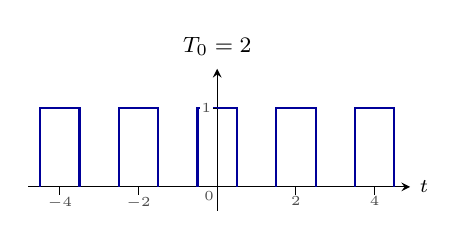
\begin{tikzpicture}[x=0.5cm,y=1.0cm]
  \taxes{-4.8}{4.9}{1.5}{-0.3}
  \foreach \c in {-4,-2,0,2,4}{\draw[sig] (\c-0.5,0) -- (\c-0.5,1) -- (\c+0.5,1) -- (\c+0.5,0);}
  \xt{2}{2}\xt{4}{4}\xt{-2}{-2}\xt{-4}{-4}\yt{1}{1}
  \node[font=\footnotesize,anchor=south] at (0,1.55) {$T_0=2$};
\end{tikzpicture}\hfill
\begin{tikzpicture}[x=0.27cm,y=1.6cm]
  \taxes[\omega]{-13.6}{13.9}{1.3}{-0.45}
  \draw[gray,dashed,domain=-12.9:12.9,samples=160] plot (\x,{sin(\x/2 r)/(\x/2)});
  \foreach \k in {-4,...,4}{%
    \pgfmathsetmacro\w{\k*pi}%
    \ifnum\k=0 \def\v{1}\else\pgfmathsetmacro\v{sin(\w/2 r)/(\w/2)}\fi
    \draw[res] (\w,0) -- (\w,\v); \fill[res] (\w,\v) circle (1.4pt);}
  \xtl{6.2832}{2\pi}{-0.32}\xtl{-6.2832}{-2\pi}{-0.32}\xtl{12.566}{4\pi}{-0.32}\xtl{-12.566}{-4\pi}{-0.32}
  \yt{1}{1}
  \node[font=\footnotesize,anchor=south] at (0,1.3) {$T_0a_k=X(jk\omega_0)$，$\omega_0=\pi$};
\end{tikzpicture}

\medskip
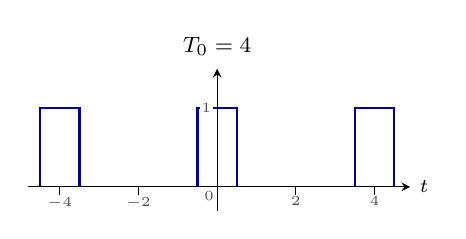
\begin{tikzpicture}[x=0.5cm,y=1.0cm]
  \taxes{-4.8}{4.9}{1.5}{-0.3}
  \foreach \c in {-4,0,4}{\draw[sig] (\c-0.5,0) -- (\c-0.5,1) -- (\c+0.5,1) -- (\c+0.5,0);}
  \xt{2}{2}\xt{4}{4}\xt{-2}{-2}\xt{-4}{-4}\yt{1}{1}
  \node[font=\footnotesize,anchor=south] at (0,1.55) {$T_0=4$};
\end{tikzpicture}\hfill
\begin{tikzpicture}[x=0.27cm,y=1.6cm]
  \taxes[\omega]{-13.6}{13.9}{1.3}{-0.45}
  \draw[gray,dashed,domain=-12.9:12.9,samples=160] plot (\x,{sin(\x/2 r)/(\x/2)});
  \foreach \k in {-8,...,8}{%
    \pgfmathsetmacro\w{\k*pi/2}%
    \ifnum\k=0 \def\v{1}\else\pgfmathsetmacro\v{sin(\w/2 r)/(\w/2)}\fi
    \draw[res] (\w,0) -- (\w,\v); \fill[res] (\w,\v) circle (1.4pt);}
  \xtl{6.2832}{2\pi}{-0.32}\xtl{-6.2832}{-2\pi}{-0.32}\xtl{12.566}{4\pi}{-0.32}\xtl{-12.566}{-4\pi}{-0.32}
  \yt{1}{1}
  \node[font=\footnotesize,anchor=south] at (0,1.3) {$T_0a_k=X(jk\omega_0)$，$\omega_0=\pi/2$};
\end{tikzpicture}
\caption{宽度为 $1$、高度为 $1$ 的方波按周期 $T_0$ 重复（左），右边红色竖线是 $T_0a_k$，画在 $k\omega_0$ 处；灰色虚线是单个方波的 $X(j\omega)=\frac{\sin(\omega/2)}{\omega/2}$。$T_0$ 从 $2$ 增大到 $4$，谱线间隔 $\omega_0$ 从 $\pi$ 缩小到 $\pi/2$，但 $T_0a_k$ 始终落在同一条曲线 $X(j\omega)$ 上。$T_0\to+\infty$ 时，只剩中间一个方波（非周期信号），谱线无限密，连成曲线 $X(j\omega)$。}
\end{figure}

\begin{note}
严格一点的说法：取一个只在有限区间内非零的非周期信号 $x(t)$，以 $T_0$ 为周期把它重复，得到周期信号 $\tilde x(t)$；只要 $T_0$ 大于 $x(t)$ 非零区间的长度，$\tilde x(t)$ 在一个周期内就等于 $x(t)$，所以一个周期上的积分与 $(-\infty,+\infty)$ 上的积分相同。上图就是这种情形。
\end{note}

%==================================================================
\section{傅里叶变换的定义}\label{sec:def}
\begin{remember}
非周期函数 $x(t)$（在 $-\infty\sim+\infty$ 上有值）的傅里叶变换，两个公式必须背下来：
\[
\begin{aligned}
X(j\omega)&=\int_{-\infty}^{+\infty}x(t)\,e^{-j\omega t}\,\dd t &&\text{（傅里叶变换）},\\
x(t)&=\frac1{2\pi}\int_{-\infty}^{+\infty}X(j\omega)\,e^{j\omega t}\,\dd\omega &&\text{（傅里叶反变换）}.
\end{aligned}
\]
\begin{itemize}[nosep]
\item $X(j\omega)$ 叫做 $x(t)$ 的\textbf{傅里叶变换}(Fourier transform)；$x(t)$ 叫做 $X(j\omega)$ 的\textbf{傅里叶反变换}(inverse Fourier transform)。
\item $x(t)$ 以时间 $t$ 为自变量，叫做\textbf{时间域}，简称\textbf{时域}(time domain)；$X(j\omega)$ 以频率 $\omega$ 为自变量，叫做\textbf{频率域}，简称\textbf{频域}(frequency domain)。
\item 四种写法，意思相同：
\[
x(t)\xrightarrow{\ \F\ }X(j\omega),\quad \F[x(t)]=X(j\omega),\quad
X(j\omega)\xrightarrow{\ \F^{-1}\ }x(t),\quad \F^{-1}[X(j\omega)]=x(t).
\]
\end{itemize}
\end{remember}

傅里叶级数针对周期信号，傅里叶变换针对非周期信号，两者的关系就是第 \ref{sec:derive} 节的推导。

%==================================================================
\section{不借助傅里叶级数：从正变换直接推出反变换}\label{sec:proof}
上面的推导要用傅里叶级数过渡。下面不用傅里叶级数，只从两个公式本身出发，看它们能不能相互推出。推一遍能加深对这两个公式的理解。

\begin{remember}
推导要用到这个公式（第一章讲 $\delta(t)$ 时强调过，后面反复用到）：
\[
\lim_{\omega\to+\infty}\frac{\sin(\omega t)}{\pi t}=\delta(t).
\]
正推、反推推不出来，很多时候是因为不知道这个公式；知道了它，就能准确地推出来。
\end{remember}

\point{题目。}若 $X(j\omega)=\displaystyle\int_{-\infty}^{+\infty}x(t)\,e^{-j\omega t}\,\dd t$，求证 $x(t)=\dfrac1{2\pi}\displaystyle\int_{-\infty}^{+\infty}X(j\omega)\,e^{j\omega t}\,\dd\omega$。

\point{证明。}从要证式子的右边出发：
\[
\text{右边}=\frac1{2\pi}\int_{-\infty}^{+\infty}X(j\omega)\,e^{j\omega t}\,\dd\omega .
\]
把 $X(j\omega)$ 的定义代进来。定义里的积分变量也叫 $t$，与这里的 $t$ 重了，所以先\textbf{换掉积分变量}，把定义里的 $t$ 换成 $u$：
\[
\text{右边}=\frac1{2\pi}\int_{-\infty}^{+\infty}\Big[\int_{-\infty}^{+\infty}x(u)\,e^{-j\omega u}\,\dd u\Big]e^{j\omega t}\,\dd\omega .
\]
\textbf{交换积分次序}：$x(u)\,\dd u$ 拿到外面，两个指数合并成 $e^{j\omega(t-u)}$：
\[
=\frac1{2\pi}\int_{-\infty}^{+\infty}x(u)\,\dd u\int_{-\infty}^{+\infty}e^{j\omega(t-u)}\,\dd\omega .
\]
先做里面对 $\omega$ 的积分，它可以直接积出来：
\[
=\frac1{2\pi}\int_{-\infty}^{+\infty}x(u)\,\dd u\Big[\frac1{j(t-u)}\,e^{j\omega(t-u)}\Big]_{\omega=-\infty}^{+\infty}.
\]
方括号里把 $\omega=+\infty$ 与 $\omega=-\infty$ 代进去相减，写成极限：
\[
\Big[\frac1{j(t-u)}\,e^{j\omega(t-u)}\Big]_{\omega=-\infty}^{+\infty}
=\frac1{j(t-u)}\lim_{\omega\to+\infty}\Big[e^{j(t-u)\omega}-e^{-j(t-u)\omega}\Big]
=\frac1{j(t-u)}\lim_{\omega\to+\infty}2j\sin[\omega(t-u)] .
\]
最后一步用了做过很多遍的公式
\[
e^{j\alpha}-e^{-j\alpha}=2j\sin\alpha,\qquad\text{（顺便记住）}\ e^{j\alpha}+e^{-j\alpha}=2\cos\alpha .
\]
$j$ 与 $j$ 约掉，$2$ 拿出来与 $\frac1{2\pi}$ 约成 $\frac1\pi$：
\[
=\frac1\pi\int_{-\infty}^{+\infty}x(u)\,\dd u\cdot\Big[\lim_{\omega\to+\infty}\frac{\sin[\omega(t-u)]}{t-u}\Big].
\]
由 $\lim\limits_{\omega\to+\infty}\frac{\sin(\omega t)}{\pi t}=\delta(t)$，把 $t$ 换成 $t-u$，得 $\lim\limits_{\omega\to+\infty}\frac{\sin[\omega(t-u)]}{t-u}=\pi\,\delta(t-u)$，所以
\[
=\frac1\pi\int_{-\infty}^{+\infty}x(u)\cdot\pi\,\delta(t-u)\,\dd u
=\int_{-\infty}^{+\infty}x(u)\,\delta(t-u)\,\dd u
=x(t).
\]
最后一步是 $\delta$ 的性质（与 $\delta$ 卷积等于自己）。所以这两个公式是相互成立的。\hfill$\square$

\example{反过来推}{由反变换推出正变换}{}
若 $x(t)=\dfrac1{2\pi}\displaystyle\int_{-\infty}^{+\infty}X(j\omega)\,e^{j\omega t}\,\dd\omega$，求证 $X(j\omega)=\displaystyle\int_{-\infty}^{+\infty}x(t)\,e^{-j\omega t}\,\dd t$。

\point{解。}步骤与上面相同。代入 $x(t)$ 时把反变换里的积分变量换成 $v$，再交换积分次序：
\[
\int_{-\infty}^{+\infty}x(t)\,e^{-j\omega t}\,\dd t
=\frac1{2\pi}\int_{-\infty}^{+\infty}X(jv)\,\dd v\int_{-\infty}^{+\infty}e^{j(v-\omega)t}\,\dd t .
\]
里面对 $t$ 的积分：
\[
\int_{-\infty}^{+\infty}e^{j(v-\omega)t}\,\dd t
=\lim_{N\to+\infty}\Big[\frac{e^{j(v-\omega)t}}{j(v-\omega)}\Big]_{t=-N}^{N}
=\lim_{N\to+\infty}\frac{2\sin[N(v-\omega)]}{v-\omega}
=2\pi\,\delta(v-\omega),
\]
最后一步同样用 $\lim\limits_{N\to+\infty}\frac{\sin(Nx)}{\pi x}=\delta(x)$。于是
\[
\int_{-\infty}^{+\infty}x(t)\,e^{-j\omega t}\,\dd t=\frac1{2\pi}\int_{-\infty}^{+\infty}X(jv)\cdot2\pi\,\delta(v-\omega)\,\dd v=X(j\omega).
\]

%==================================================================
\section{七个典型傅里叶变换对}\label{sec:seven}
连续时间信号的傅里叶变换（教材 3.2.3 节）是整门课的重点：后面信号与系统的学习基本上都依靠这里。不要把它看成例题，而要看成必须背下来的东西。左边是时域（以 $t$ 为自变量），右边是频域（以 $\omega$ 为自变量），一左一右叫做一个\textbf{傅里叶变换对}(Fourier transform pair)。

\begin{remember}
七个公式全部记住：
\begin{center}
\renewcommand{\arraystretch}{1.9}
\begin{tabular}{c>{$\displaystyle}r<{$}c>{$\displaystyle}l<{$}l}
\toprule
编号 & \text{时域 }x(t) & & \text{频域 }X(j\omega) & 备注\\
\midrule
\textcircled{\scriptsize 1} & e^{-at}u(t) & $\xrightarrow{\F}$ & \frac1{a+j\omega} & 只对 $a>0$ 成立\\
\textcircled{\scriptsize 2} & \delta(t) & $\xrightarrow{\F}$ & 1 & \textcircled{\scriptsize 2} 与 \textcircled{\scriptsize 3} 一对\\
\textcircled{\scriptsize 3} & 1 & $\xrightarrow{\F}$ & 2\pi\,\delta(\omega) & \\
\textcircled{\scriptsize 4} & \text{方波：}-\tfrac\tau2\sim\tfrac\tau2\text{ 上高 }E & $\xrightarrow{\F}$ & E\tau\Sa\Big(\frac\tau2\omega\Big)=\frac{2E\sin(\frac\tau2\omega)}{\omega} & \textcircled{\scriptsize 4} 与 \textcircled{\scriptsize 5} 一对\\
\textcircled{\scriptsize 5} & \frac{\sin(\omega_ct)}{\pi t} & $\xrightarrow{\F}$ & \text{方波：}-\omega_c\sim\omega_c\text{ 上高 }1 & \\
\textcircled{\scriptsize 6} & u(t) & $\xrightarrow{\F}$ & \frac1{j\omega}+\pi\,\delta(\omega) & \\
\textcircled{\scriptsize 7} & \cos(\omega_0t) & $\xrightarrow{\F}$ & \pi\big[\delta(\omega+\omega_0)+\delta(\omega-\omega_0)\big] & 两个合成一条记\\
 & \sin(\omega_0t) & $\xrightarrow{\F}$ & \frac\pi j\big[\delta(\omega-\omega_0)-\delta(\omega+\omega_0)\big] & \\
\bottomrule
\end{tabular}
\end{center}
\end{remember}

对每一个变换对，除了公式，还要对时域和频域的\textbf{形状}了如指掌，所以下面每一个都把时域和频域画出来。

%------------------------------------------------------------------
\subsection{\texorpdfstring{\textcircled{\scriptsize 1} 单边指数信号 $e^{-at}u(t)$}{① 单边指数信号}}\label{sub:exp}
\begin{remember}
\[
e^{-at}u(t)\ \xrightarrow{\ \F\ }\ \frac1{a+j\omega}\qquad(a>0).
\]
\end{remember}

\point{推导。}代入正变换公式：
\[
X(j\omega)=\int_{-\infty}^{+\infty}x(t)\,e^{-j\omega t}\,\dd t=\int_{-\infty}^{+\infty}e^{-at}u(t)\,e^{-j\omega t}\,\dd t .
\]
$u(t)$ 在 $t>0$ 时为 $1$、$t<0$ 时为 $0$，乘上 $u(t)$ 后，$t<0$ 那一半全变成 $0$，不用考虑，积分限变成 $0\sim+\infty$。再把 $e^{-at}$ 与 $e^{-j\omega t}$ 合并：
\[
X(j\omega)=\int_0^{+\infty}e^{-(a+j\omega)t}\,\dd t
=-\frac1{a+j\omega}\,e^{-(a+j\omega)t}\Big|_{t=0}^{+\infty}
=-\frac1{a+j\omega}\Big[e^{-(a+j\omega)\cdot(+\infty)}-1\Big].
\]
$t=0$ 代入，$e^0=1$。$a$ 是实数，\textbf{当且仅当 $a>0$ 时}，$-a$ 乘以 $+\infty$ 得 $-\infty$，第一项为 $0$；两个负号抵消，
\[
X(j\omega)=\frac1{a+j\omega}.
\]
若 $a<0$，第一项是 $e$ 的正无穷大次方，根本不收敛，没有傅里叶变换。所以这个公式只对 $a>0$ 成立。

\point{时域形状。}乘了 $u(t)$，负的那一半全是 $0$；从 $t=0$ 处的 $1$ 开始，$a>0$ 所以向右衰减。$a$ 越大，衰减越快（下图左，$a_2>a_1$）。

\point{频域：幅度谱与相位谱。}$X(j\omega)=\frac1{a+j\omega}$ 含有虚数单位 $j$，没法直接画在一张图上，要把一幅图拆成两幅。可以分成实部与虚部：
\[
\frac1{a+j\omega}=\frac{a-j\omega}{(a+j\omega)(a-j\omega)}=\frac{a-j\omega}{a^2+\omega^2}=\frac{a}{a^2+\omega^2}-j\,\frac{\omega}{a^2+\omega^2},
\]
先画实部、再画虚部。但在频域上一般不这样画，而是写成模与相位：
\[
X(j\omega)=|X(j\omega)|\,e^{j\theta(\omega)},
\]
$|X(j\omega)|$ 叫做\textbf{幅度谱}(amplitude spectrum)，$\theta(\omega)$ 叫做\textbf{相位谱}(phase spectrum)。

求模与相位只需要两个高中公式：对复数 $z=a+jb$，
\[
|z|=\sqrt{a^2+b^2},\qquad \theta=\arctan\frac ba .
\]
$X(j\omega)=\frac1{a+j\omega}$ 的分子是 $1$，模就是分母的模取倒数，相位是分母相位取负号（$\arctan$ 是奇函数）：
\[
|X(j\omega)|=\frac1{\sqrt{a^2+\omega^2}},\qquad
\theta(\omega)=\arctan\Big(-\frac\omega a\Big)=-\arctan\frac\omega a .
\]
\begin{itemize}[nosep]
\item 幅度谱：$\omega=0$ 时为 $\frac1a$；左右对称；$|\omega|$ 越大越趋于 $0$。
\item 相位谱：$\omega\to+\infty$ 时趋于 $-\frac\pi2$；$\omega\to-\infty$ 时（$-\omega$ 取正值，负负得正）趋于 $+\frac\pi2$。
\end{itemize}

\begin{figure}[H]
\centering
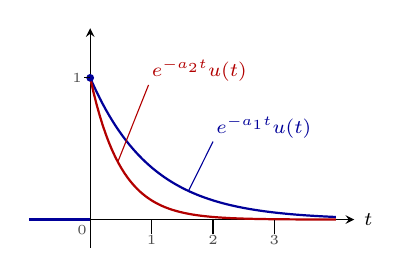
\begin{tikzpicture}[x=0.78cm,y=1.8cm]
  \taxes{-1.0}{4.3}{1.35}{-0.2}
  \draw[sig] (-1.0,0) -- (0,0);
  \draw[sig,domain=0:4,samples=80] plot (\x,{exp(-\x)});
  \draw[res,domain=0:4,samples=80] plot (\x,{exp(-2*\x)});
  \fill[blue!60!black] (0,1) circle (1.4pt);
  \xt{1}{1}\xt{2}{2}\xt{3}{3}\yt{1}{1}
  \draw[blue!60!black,thin] (1.6,0.202) -- (2.0,0.55) node[anchor=south west,inner sep=1pt,font=\scriptsize] {$e^{-a_1t}u(t)$};
  \draw[red!70!black,thin] (0.45,0.407) -- (0.95,0.95) node[anchor=south west,inner sep=1pt,font=\scriptsize] {$e^{-a_2t}u(t)$};
\end{tikzpicture}\hfill
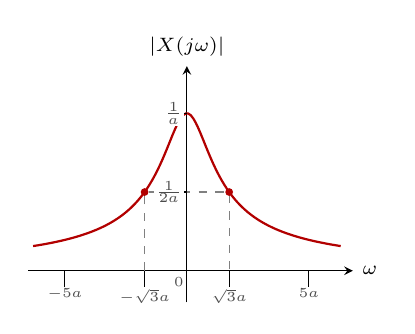
\begin{tikzpicture}[x=0.31cm,y=2.0cm]
  \taxes[\omega]{-6.5}{6.8}{1.3}{-0.2}
  \draw[res,domain=-6.3:6.3,samples=120] plot (\x,{1/sqrt(1+\x*\x)});
  \draw[gray,dashed] (-1.732,0) -- (-1.732,0.5) -- (1.732,0.5) -- (1.732,0);
  \fill[red!70!black] (1.732,0.5) circle (1.4pt) (-1.732,0.5) circle (1.4pt);
  \xt{1.732}{\sqrt3a}\xt{-1.732}{-\sqrt3a}\xt{5}{5a}\xt{-5}{-5a}
  \yt{1}{\frac1a}\yt{0.5}{\frac1{2a}}
  \node[font=\scriptsize,anchor=south] at (0,1.3) {$|X(j\omega)|$};
\end{tikzpicture}\hfill
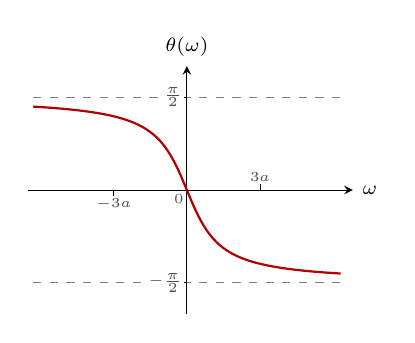
\begin{tikzpicture}[x=0.31cm,y=0.75cm]
  \taxes[\omega]{-6.5}{6.8}{2.1}{-2.1}
  \draw[gray,dashed] (-6.3,1.5708) -- (6.3,1.5708) (-6.3,-1.5708) -- (6.3,-1.5708);
  \draw[res,domain=-6.3:6.3,samples=120] plot (\x,{-atan(\x)*pi/180});
  \yt{1.5708}{\frac\pi2}\yt{-1.5708}{-\frac\pi2}
  \xtu{3}{3a}\xt{-3}{-3a}
  \node[font=\scriptsize,anchor=south] at (0,2.1) {$\theta(\omega)$};
\end{tikzpicture}
\caption{左：$e^{-at}u(t)$，$a_2=2a_1$，$a$ 越大衰减越快；$t<0$ 时为 $0$。中：幅度谱 $|X(j\omega)|=\frac1{\sqrt{a^2+\omega^2}}$（画图取 $a=1$），峰值 $\frac1a$，在 $\omega=\pm\sqrt3a$ 处降到峰值的一半 $\frac1{2a}$。右：相位谱 $\theta(\omega)=-\arctan\frac\omega a$，从 $+\frac\pi2$ 单调降到 $-\frac\pi2$，过原点。}
\end{figure}

\point{低通滤波器。}这样的幅度谱叫做\textbf{低通滤波器}(low-pass filter)：$|\omega|$ 很小的地方幅度比较大，$|\omega|$ 很大的地方幅度比较小。频率就是 $\omega$，它让频率较低的部分通过，把频率较高的部分抑制住。后面讲滤波器分析和设计时还会深入讲。

\point{截止频率。}幅度衰减为最高幅度一半时的频率，叫做\textbf{滤波器的截止频率}(cutoff frequency)（低通、高通、带通都一样）。幅度衰减到最高点的一半，也叫\textbf{幅度衰减 3\,dB}。dB 叫分贝(decibel)，它不以幅度本身为单位，而是取对数再乘 $10$：
\[
10\lg|X(j\omega)|\ \text{dB},\qquad -10\lg\frac12\approx3 .
\]
对 $e^{-at}u(t)$：把 $\omega=\sqrt3a$ 代入，$|X(j\omega)|=\frac1{\sqrt{a^2+3a^2}}=\frac1{2a}$，正好是峰值 $\frac1a$ 的一半（$\omega=-\sqrt3a$ 处也一样），所以它的截止频率为 $\sqrt3a$。

\begin{note}
工程上更常用的约定：幅度的分贝数用 $20\lg|X(j\omega)|$（$10\lg$ 用于功率，功率与幅度的平方成正比）。按这个约定，「衰减 3\,dB」是\textbf{功率}降为一半、\textbf{幅度}降为最高点的 $\frac1{\sqrt2}\approx0.707$；幅度降为一半对应约 $6$\,dB。按 $\frac1{\sqrt2}$ 计算，$\frac1{\sqrt{a^2+\omega^2}}=\frac1{\sqrt2\,a}$ 解出 $\omega=a$，即 $e^{-at}u(t)$ 的 3\,dB 截止频率为 $a$。读其他教材或滤波器资料时，截止频率一般指这个值。
\end{note}

%------------------------------------------------------------------
\subsection{\texorpdfstring{\textcircled{\scriptsize 2} 冲激 $\delta(t)$}{② 冲激 δ(t)}}\label{sub:delta}
\begin{remember}
\[
\delta(t)\ \xrightarrow{\ \F\ }\ 1 .
\]
\end{remember}
\point{证明。}代入正变换公式，并用 $\delta$ 性质中最重要的一条 $\displaystyle\int_{-\infty}^{+\infty}x(t)\,\delta(t)\,\dd t=x(0)$：
\[
X(j\omega)=\int_{-\infty}^{+\infty}\delta(t)\,e^{-j\omega t}\,\dd t=e^{-j\omega\cdot0}=1 .
\]
时域是原点处的一个冲激，频域是一条处处为 $1$ 的水平线（下图上排）。

%------------------------------------------------------------------
\subsection{\texorpdfstring{\textcircled{\scriptsize 3} 常数 $1$}{③ 常数 1}}\label{sub:one}
\begin{remember}
\[
1\ \xrightarrow{\ \F\ }\ 2\pi\,\delta(\omega).
\]
\end{remember}
有简单做法和复杂做法：从右边推回左边（用反变换公式）是简单做法；从左边推到右边是复杂做法。

\point{简单做法：右推左。}代入反变换公式：
\[
x(t)=\frac1{2\pi}\int_{-\infty}^{+\infty}X(j\omega)\,e^{j\omega t}\,\dd\omega
=\frac1{2\pi}\int_{-\infty}^{+\infty}2\pi\,\delta(\omega)\,e^{j\omega t}\,\dd\omega
=\int_{-\infty}^{+\infty}\delta(\omega)\,e^{j\omega t}\,\dd\omega .
\]
还是用 $\int x(t)\delta(t)\,\dd t=x(0)$，但要注意公式的自变量：把公式里的自变量全部换成 $\omega$，
\[
\int_{-\infty}^{+\infty}x(\omega)\,\delta(\omega)\,\dd\omega=x(0),
\]
这里 $x(\omega)=e^{j\omega t}$ 是 $\omega$ 的函数，于是
\[
x(t)=e^{j\cdot0\cdot t}=1 .
\]

\point{复杂做法：左推右。}代入正变换公式，$x(t)$ 恒等于 $1$。把 $-\infty\sim+\infty$ 写成 $-N\sim N$ 再令 $N\to+\infty$：
\[
\begin{aligned}
X(j\omega)&=\int_{-\infty}^{+\infty}1\cdot e^{-j\omega t}\,\dd t
=\lim_{N\to+\infty}\int_{-N}^{N}e^{-j\omega t}\,\dd t
=\lim_{N\to+\infty}-\frac1{j\omega}\,e^{-j\omega t}\Big|_{-N}^{N}\\
&=\lim_{N\to+\infty}\frac1{j\omega}\big(e^{j\omega N}-e^{-j\omega N}\big).
\end{aligned}
\]
最后一步把前面的负号去掉、括号里两项交换顺序。括号里用 $e^{j\alpha}-e^{-j\alpha}=2j\sin\alpha$，$j$ 与 $j$ 约掉：
\[
X(j\omega)=\lim_{N\to+\infty}\frac{2\sin(\omega N)}{\omega}=2\pi\,\delta(\omega).
\]
最后一步来自公式 $\lim\limits_{\omega\to+\infty}\frac{\sin(\omega t)}{\pi t}=\delta(t)$：把其中的 $t$ 换成 $\omega$、$\omega$ 换成 $N$，就是 $\lim\limits_{N\to+\infty}\frac{\sin(N\omega)}{\pi\omega}=\delta(\omega)$，即 $\lim\limits_{N\to+\infty}\frac{\sin(N\omega)}{\omega}=\pi\,\delta(\omega)$。这个公式只是把变量换来换去而已。所以左推右、右推左都可以。

\begin{figure}[H]
\centering
\begin{tikzpicture}[x=0.75cm,y=1.0cm]
  \taxes{-2.6}{2.8}{1.5}{-0.25}
  \draw[sig,imp] (0,0) -- (0,1.1);
  \node[font=\scriptsize,blue!60!black,anchor=west] at (0.08,1.1) {$(1)$};
  \xt{1}{1}\xt{2}{2}\xt{-1}{-1}\xt{-2}{-2}
  \node[font=\scriptsize,anchor=south] at (0,1.5) {$\delta(t)$};
\end{tikzpicture}
\quad$\xrightarrow{\ \F\ }$\quad
\begin{tikzpicture}[x=0.75cm,y=1.0cm]
  \taxes[\omega]{-2.6}{2.8}{1.5}{-0.25}
  \draw[res] (-2.5,0.8) -- (2.5,0.8);
  \xt{1}{1}\xt{2}{2}\xt{-1}{-1}\xt{-2}{-2}\yt{0.8}{1}
  \node[font=\scriptsize,anchor=south] at (0,1.5) {$X(j\omega)=1$};
\end{tikzpicture}

\medskip
\begin{tikzpicture}[x=0.75cm,y=1.0cm]
  \taxes{-2.6}{2.8}{1.5}{-0.25}
  \draw[sig] (-2.5,0.8) -- (2.5,0.8);
  \xt{1}{1}\xt{2}{2}\xt{-1}{-1}\xt{-2}{-2}\yt{0.8}{1}
  \node[font=\scriptsize,anchor=south] at (0,1.5) {$x(t)=1$};
\end{tikzpicture}
\quad$\xrightarrow{\ \F\ }$\quad
\begin{tikzpicture}[x=0.75cm,y=1.0cm]
  \taxes[\omega]{-2.6}{2.8}{1.5}{-0.25}
  \draw[res,imp] (0,0) -- (0,1.1);
  \node[font=\scriptsize,red!70!black,anchor=west] at (0.08,1.1) {$(2\pi)$};
  \xt{1}{1}\xt{2}{2}\xt{-1}{-1}\xt{-2}{-2}
  \node[font=\scriptsize,anchor=south] at (0,1.5) {$2\pi\,\delta(\omega)$};
\end{tikzpicture}
\caption{上：$\delta(t)$ 的傅里叶变换是处处为 $1$ 的常数。下：常数 $1$ 的傅里叶变换是 $\omega=0$ 处强度为 $2\pi$ 的冲激（括号里是冲激的强度）。两对互为镜像：时域越「窄」（冲激），频域越「宽」（常数），反之亦然。}
\end{figure}

\point{\textcircled{\scriptsize 2} 与 \textcircled{\scriptsize 3} 是一对。}它们的推法类似：\textcircled{\scriptsize 2} 上面用的是左推右，\textcircled{\scriptsize 2} 的右推左与 \textcircled{\scriptsize 3} 的左推右做法一样，留作练习。

\example{\textcircled{\scriptsize 2} 的右推左}{$\frac1{2\pi}\int e^{j\omega t}\dd\omega=\delta(t)$}{}
代入反变换公式，同样把 $-\infty\sim+\infty$ 写成 $-N\sim N$：
\[
\begin{aligned}
x(t)&=\frac1{2\pi}\int_{-\infty}^{+\infty}1\cdot e^{j\omega t}\,\dd\omega
=\frac1{2\pi}\lim_{N\to+\infty}\frac{e^{jNt}-e^{-jNt}}{jt}\\
&=\frac1{2\pi}\lim_{N\to+\infty}\frac{2\sin(Nt)}{t}
=\lim_{N\to+\infty}\frac{\sin(Nt)}{\pi t}=\delta(t).
\end{aligned}
\]

%------------------------------------------------------------------
\subsection{\texorpdfstring{\textcircled{\scriptsize 4} 方波（矩形窗函数）}{④ 方波（矩形窗函数）}}\label{sub:rect}
\begin{remember}
时域是 $-\frac\tau2\sim\frac\tau2$ 上高为 $E$ 的方波（矩形窗函数），
\[
\text{方波}\ \xrightarrow{\ \F\ }\ E\tau\Sa\Big(\frac\tau2\omega\Big)=\frac{2E\sin(\frac\tau2\omega)}{\omega},
\qquad \Sa(x)=\frac{\sin x}{x}.
\]
\end{remember}
化简：$E\tau\Sa(\frac\tau2\omega)=E\tau\cdot\frac{\sin(\frac\tau2\omega)}{\frac\tau2\omega}$，$2$ 翻上去、$\tau$ 与 $\tau$ 约掉，得 $\frac{2E\sin(\frac\tau2\omega)}{\omega}$。

\point{推导：左推右。}方波只在 $-\frac\tau2\sim\frac\tau2$ 上有值（值为 $E$），两边全是 $0$，积分限直接缩成 $-\frac\tau2\sim\frac\tau2$：
\[
X(j\omega)=\int_{-\tau/2}^{\tau/2}E\,e^{-j\omega t}\,\dd t
=E\cdot\Big(-\frac1{j\omega}\Big)e^{-j\omega t}\Big|_{t=-\tau/2}^{\tau/2}
=\frac E{j\omega}\Big(e^{j\omega\frac\tau2}-e^{-j\omega\frac\tau2}\Big)
\]
（负号去掉、两项交换）。再用 $e^{j\alpha}-e^{-j\alpha}=2j\sin\alpha$，$j$ 与 $j$ 约掉：
\[
X(j\omega)=\frac{E\cdot2j\sin(\omega\frac\tau2)}{j\omega}=\frac{2E\sin(\omega\frac\tau2)}{\omega}=E\tau\Sa\Big(\omega\frac\tau2\Big).
\]

\begin{figure}[H]
\centering
\begin{tikzpicture}[x=0.9cm,y=1.1cm]
  \taxes{-2.6}{2.8}{1.5}{-0.3}
  \draw[sig] (-2.5,0) -- (-1,0) -- (-1,1) -- (1,1) -- (1,0) -- (2.5,0);
  \xt{-1}{-\frac\tau2}\xt{1}{\frac\tau2}\yt{1}{E}
\end{tikzpicture}
\quad$\xrightarrow{\ \F\ }$\quad
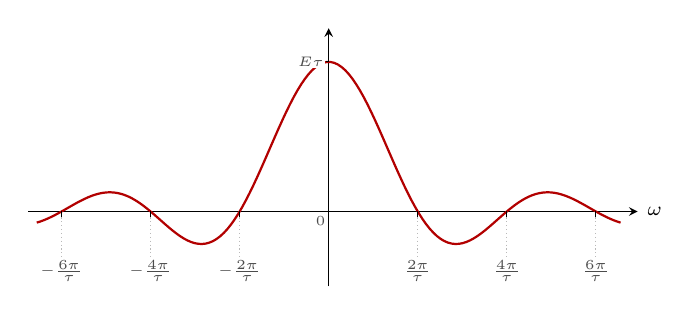
\begin{tikzpicture}[x=0.36cm,y=0.95cm]
  \taxes[\omega]{-10.6}{10.9}{2.45}{-1.0}
  \draw[res,domain=-10.3:10.3,samples=160] plot (\x,{2*sin(\x r)/\x});
  \xtl{3.1416}{\frac{2\pi}\tau}{-0.62}\xtl{-3.1416}{-\frac{2\pi}\tau}{-0.62}
  \xtl{6.2832}{\frac{4\pi}\tau}{-0.62}\xtl{-6.2832}{-\frac{4\pi}\tau}{-0.62}
  \xtl{9.4248}{\frac{6\pi}\tau}{-0.62}\xtl{-9.4248}{-\frac{6\pi}\tau}{-0.62}
  \yt{2}{E\tau}
\end{tikzpicture}
\caption{左：$-\frac\tau2\sim\frac\tau2$ 上高 $E$ 的方波（画图取 $E=1$、$\tau=2$）。右：它的傅里叶变换 $E\tau\Sa(\frac\tau2\omega)$，峰值 $E\tau$ 正好是方波的面积，过零点在 $\omega=\pm\frac{2\pi}\tau,\pm\frac{4\pi}\tau,\dots$，即 $\frac\tau2\omega=\pm\pi,\pm2\pi,\dots$。方波越宽（$\tau$ 越大），Sa 越窄越高。}
\end{figure}

%------------------------------------------------------------------
\subsection{\texorpdfstring{\textcircled{\scriptsize 5} $\frac{\sin(\omega_ct)}{\pi t}$}{⑤ sin(ωc t)/(πt)}}\label{sub:sinc}
\begin{remember}
\[
\frac{\sin(\omega_ct)}{\pi t}\ \xrightarrow{\ \F\ }\ \text{频域上 }-\omega_c\sim\omega_c\text{ 上高为 }1\text{ 的方波}\qquad(\omega_c>0).
\]
\end{remember}
\textcircled{\scriptsize 4} 与 \textcircled{\scriptsize 5} 说的是同一句话：
\begin{remember}
\textbf{方波与 Sa 互为傅里叶变换。}时域是方波，频域是 Sa；时域是 Sa，频域是方波。这个结论是后面采样定理、低通滤波器等内容的重要基础。
\end{remember}

\point{推导：左推右。}教材上推的是右推左（比较好推）。这里做左推右：
\[
X(j\omega)=\int_{-\infty}^{+\infty}\frac{\sin(\omega_ct)}{\pi t}\,e^{-j\omega t}\,\dd t
=\int_{-\infty}^{+\infty}\frac{\sin(\omega_ct)}{\pi t}\big[\cos(\omega t)-j\sin(\omega t)\big]\dd t ,
\]
老老实实拆成两项：
\[
X(j\omega)=\int_{-\infty}^{+\infty}\frac{\sin(\omega_ct)}{\pi t}\cos(\omega t)\,\dd t
-j\int_{-\infty}^{+\infty}\frac{\sin(\omega_ct)}{\pi t}\sin(\omega t)\,\dd t .
\]
\textbf{学傅里叶级数、傅里叶变换时，要随时随地关注奇偶性。}第二项直接等于 $0$：$\sin(\omega_ct)$ 是奇函数，$t$ 是奇函数，相除是偶函数；再乘以奇函数 $\sin(\omega t)$，整个被积函数是 $t$ 的奇函数。任何一个奇函数在 $-\infty\sim+\infty$（左右对称的区间）上的积分都等于 $0$。

第一项用积化和差 $\sin\alpha\cos\beta=\frac12\big[\sin(\alpha+\beta)+\sin(\alpha-\beta)\big]$，拆成两项：
\[
X(j\omega)=\frac12\Big[\int_{-\infty}^{+\infty}\frac{\sin[(\omega_c+\omega)t]}{\pi t}\,\dd t+\int_{-\infty}^{+\infty}\frac{\sin[(\omega_c-\omega)t]}{\pi t}\,\dd t\Big].
\]
再用第一章的公式：
\[
\int_{-\infty}^{+\infty}\frac{\sin(\omega t)}{\pi t}\,\dd t=\begin{cases}1, & \omega>0,\\ -1, & \omega<0 .\end{cases}
\]
分三种情况讨论（前提条件 $\omega_c>0$）：
\begin{enumerate}[nosep,label=\textcircled{\scriptsize\arabic*}]
\item 当 $\omega<-\omega_c$ 时：$\omega+\omega_c<0$，$\omega_c-\omega>0$，上式 $=\frac12[-1+1]=0$；
\item 当 $-\omega_c<\omega<\omega_c$ 时：$\omega_c+\omega>0$，$\omega_c-\omega>0$，上式 $=\frac12[1+1]=1$；
\item 当 $\omega>\omega_c$ 时：$\omega_c+\omega>0$，$\omega_c-\omega<0$，上式 $=\frac12[1-1]=0$。
\end{enumerate}
总结起来，$X(j\omega)$ 只在 $-\omega_c\sim\omega_c$ 上等于 $1$，其余为 $0$，就是一个方波。

\begin{figure}[H]
\centering
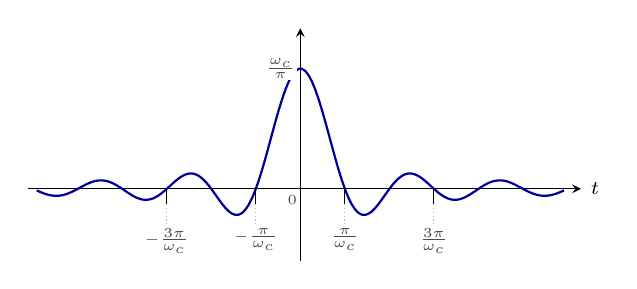
\begin{tikzpicture}[x=0.36cm,y=2.4cm]
  \taxes{-9.6}{9.9}{0.85}{-0.38}
  \draw[sig,domain=-9.3:9.3,samples=160] plot (\x,{sin(2*\x r)/(pi*\x)});
  \xtl{1.5708}{\frac\pi{\omega_c}}{-0.2}\xtl{-1.5708}{-\frac\pi{\omega_c}}{-0.2}
  \xtl{4.7124}{\frac{3\pi}{\omega_c}}{-0.2}\xtl{-4.7124}{-\frac{3\pi}{\omega_c}}{-0.2}
  \yt{0.6366}{\frac{\omega_c}\pi}
\end{tikzpicture}
\quad$\xrightarrow{\ \F\ }$\quad
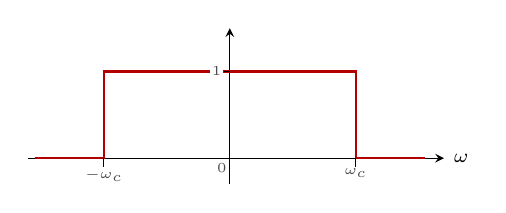
\begin{tikzpicture}[x=0.8cm,y=1.1cm]
  \taxes[\omega]{-3.2}{3.4}{1.5}{-0.3}
  \draw[res] (-3.1,0) -- (-2,0) -- (-2,1) -- (2,1) -- (2,0) -- (3.1,0);
  \xt{-2}{-\omega_c}\xt{2}{\omega_c}\yt{1}{1}
\end{tikzpicture}
\caption{左：$\frac{\sin(\omega_ct)}{\pi t}$（画图取 $\omega_c=2$），峰值 $\frac{\omega_c}\pi$，过零点 $\pm\frac{\pi}{\omega_c},\pm\frac{2\pi}{\omega_c},\dots$。右：它的傅里叶变换是 $-\omega_c\sim\omega_c$ 上高为 $1$ 的方波。与上一张图对照：方波与 Sa 的位置在时域、频域之间互换。}
\end{figure}

\point{另外两个方向。}\textcircled{\scriptsize 4} 的右推左与 \textcircled{\scriptsize 5} 的左推右所用的原理完全一样；\textcircled{\scriptsize 5} 的右推左与 \textcircled{\scriptsize 4} 的左推右所用的原理完全一样。两者都留作练习。

\example{\textcircled{\scriptsize 5} 的右推左}{与 \textcircled{\scriptsize 4} 的左推右同理}{}
\[
x(t)=\frac1{2\pi}\int_{-\omega_c}^{\omega_c}1\cdot e^{j\omega t}\,\dd\omega
=\frac1{2\pi}\cdot\frac{e^{j\omega_ct}-e^{-j\omega_ct}}{jt}
=\frac1{2\pi}\cdot\frac{2\sin(\omega_ct)}{t}=\frac{\sin(\omega_ct)}{\pi t}.
\]

\example{\textcircled{\scriptsize 4} 的右推左}{与 \textcircled{\scriptsize 5} 的左推右同理}{}
\[
x(t)=\frac1{2\pi}\int_{-\infty}^{+\infty}\frac{2E\sin(\frac\tau2\omega)}{\omega}\big[\cos(\omega t)+j\sin(\omega t)\big]\dd\omega .
\]
虚部的被积函数是 $\omega$ 的奇函数（偶 $\times$ 奇），积分为 $0$。实部积化和差：
\[
x(t)=\frac E{2\pi}\Big[\int_{-\infty}^{+\infty}\frac{\sin[(\frac\tau2+t)\omega]}{\omega}\,\dd\omega+\int_{-\infty}^{+\infty}\frac{\sin[(\frac\tau2-t)\omega]}{\omega}\,\dd\omega\Big],
\]
每个积分按系数的正负等于 $\pm\pi$。$|t|<\frac\tau2$ 时两个系数都为正，$x(t)=\frac E{2\pi}(\pi+\pi)=E$；$|t|>\frac\tau2$ 时一正一负，$x(t)=0$。正是方波。

%------------------------------------------------------------------
\subsection{方波与 Sa：快速写出变换}\label{sub:fast}
\textcircled{\scriptsize 4} 和 \textcircled{\scriptsize 5} 不是要生硬地记公式，而是要能非常快地写出方波与 Sa 之间的正变换、反变换。后面的推导会频繁用到它们。

\point{为什么系数是面积。}方波的变换写成 $A\Sa(c\,\omega)$ 的形式，$A$ 等于多少？在正变换公式里令 $\omega=0$：
\[
X(j0)=\int_{-\infty}^{+\infty}x(t)\,e^{-j\cdot0\cdot t}\,\dd t=\int_{-\infty}^{+\infty}x(t)\,\dd t ,
\]
$e^0=1$，所以 $X(j0)$ 就是 $x(t)$ 的积分，也就是\textbf{时域的面积}。另一方面 $X(j0)=A\Sa(0)=A$（$\Sa(0)=\lim\limits_{t\to0}\frac{\sin t}{t}=1$）。所以 $A$ = 方波的面积。

\point{反过来：方波的高度。}在反变换公式里令 $t=0$：
\[
x(0)=\frac1{2\pi}\int_{-\infty}^{+\infty}X(j\omega)\,e^{j\omega\cdot0}\,\dd\omega=\frac1{2\pi}\int_{-\infty}^{+\infty}X(j\omega)\,\dd\omega ,
\]
即\textbf{时域在 $0$ 处的值 = 频域的面积除以 $2\pi$}。方波在 $0$ 处的值就是它的高度。

频域面积要用第一章的公式
\[
\int_{-\infty}^{+\infty}\frac{\sin(\omega t)}{t}\,\dd t=\pi\quad(\omega>0),
\]
把 $\omega$ 和 $t$ 整个互换，得
\[
\int_{-\infty}^{+\infty}\frac{\sin(t\,\omega)}{\omega}\,\dd\omega=\pi\quad(t>0).
\]
例如 $\displaystyle\int_{-\infty}^{+\infty}\frac{\sin(3\omega)}{\omega}\,\dd\omega=\pi$：分子里 $\omega$ 的系数是多少都一样，积分都是 $\pi$。

\begin{remember}
\begin{itemize}[nosep]
\item $X(j0)=\displaystyle\int_{-\infty}^{+\infty}x(t)\,\dd t$：频域在 $0$ 处的值 = 时域面积。
\item $x(0)=\dfrac1{2\pi}\displaystyle\int_{-\infty}^{+\infty}X(j\omega)\,\dd\omega$：时域在 $0$ 处的值 = 频域面积 $/2\pi$。
\item $\displaystyle\int_{-\infty}^{+\infty}\frac{\sin(ct)}{t}\,\dd t=\pi$（$c>0$），把 $t$ 换成 $\omega$ 也一样。
\end{itemize}
\end{remember}

\subsection{做题步骤}\label{sub:steps}
\point{时域方波 $\to$ 频域 Sa。}
\begin{enumerate}[nosep]
\item 方波对应 Sa，先写出 $\Sa(\ \cdot\ \omega)$：时域自变量是 $t$，频域自变量是 $\omega$，所以 Sa 里必然有一个 $\omega$。
\item Sa 括号里 $\omega$ 的系数 = 方波的截止点（半宽）。
\item Sa 前面的系数 = 方波的面积。
\item 需要时化简：$A\Sa(c\omega)=\frac{A\sin(c\omega)}{c\omega}$。
\end{enumerate}

\point{频域 Sa $\to$ 时域方波。}
\begin{enumerate}[nosep]
\item 先认出它是 Sa：只要是 $\sin(\ \cdot\ \omega)$ 且分母也有一个 $\omega$，就一定是 Sa，哪怕没有显式写成 $\Sa$。它对应时域方波，先把方波画出来。
\item 方波的截止点 = $\sin$ 括号里 $\omega$ 的系数。
\item 方波的高度 = $x(0)$ = 频域面积 $/2\pi$；频域面积用 $\int\frac{\sin(c\omega)}{\omega}\,\dd\omega=\pi$ 一眼看出。
\end{enumerate}

\point{时域 $\frac{\sin(ct)}{kt}$ $\to$ 频域方波。}截止点为 $\pm c$；高度 $=X(j0)=\int\frac{\sin(ct)}{kt}\,\dd t=\frac\pi k$。

\point{频域方波 $\to$ 时域。}$-c\sim c$ 上高为 $H$ 的方波，对应 $\frac{H\sin(ct)}{\pi t}$（由 \textcircled{\scriptsize 5}，除以 $\pi t$ 后，高度 $1$ 对应系数 $1$）。

\point{易错点。}$\Sa$ 与 $\sin$ 不同：$\Sa(3\omega)=\frac{\sin(3\omega)}{3\omega}$，不能把 $12\Sa(3\omega)$ 写成 $12\sin(3\omega)$。

\begin{figure}[H]
\centering
\begin{tikzpicture}[x=0.42cm,y=0.65cm]
  \taxes{-4.8}{5.0}{2.6}{-0.4}
  \draw[sig] (-4.7,0) -- (-3,0) -- (-3,2) -- (3,2) -- (3,0) -- (4.7,0);
  \fill[blue!12] (-3,0) rectangle (3,2);
  \draw[sig] (-3,0) -- (-3,2) -- (3,2) -- (3,0);
  \node[font=\scriptsize,blue!60!black] at (1.5,1.0) {面积 $12$};
  \xt{-3}{-3}\xt{3}{3}\yt{2}{2}
\end{tikzpicture}
\quad$\xrightarrow{\ \F\ }$\quad
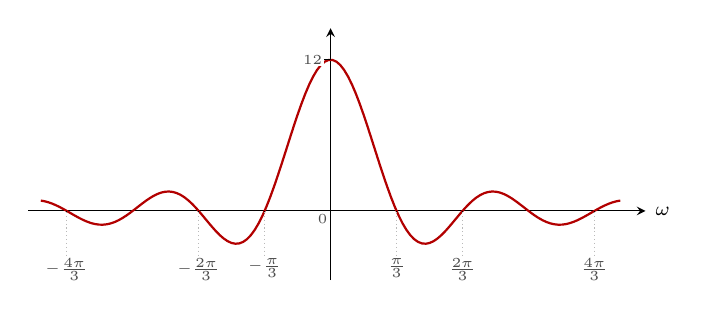
\begin{tikzpicture}[x=0.8cm,y=0.16cm]
  \taxes[\omega]{-4.8}{5.0}{14.5}{-5.5}
  \draw[res,domain=-4.6:4.6,samples=150] plot (\x,{4*sin(3*\x r)/\x});
  \xtl{1.0472}{\frac\pi3}{-3.6}\xtl{-1.0472}{-\frac\pi3}{-3.6}\xtl{2.0944}{\frac{2\pi}3}{-3.6}\xtl{-2.0944}{-\frac{2\pi}3}{-3.6}
  \xtl{4.1888}{\frac{4\pi}3}{-3.6}\xtl{-4.1888}{-\frac{4\pi}3}{-3.6}
  \yt{12}{12}
\end{tikzpicture}
\caption{例 \ref{ex:r1} 的方波（$-3\sim3$ 上高 $2$）与它的傅里叶变换 $12\Sa(3\omega)=\frac{4\sin(3\omega)}{\omega}$：频域在 $\omega=0$ 处的值 $12$ 正好等于时域方波的面积 $2\times6$；Sa 里的系数 $3$ 就是方波的截止点，过零点在 $\omega=\pm\frac\pi3,\pm\frac{2\pi}3,\dots$。}
\end{figure}

\subsection{例题}\label{sub:ex}
\example{方波 $\to$ Sa}{$12\Sa(3\omega)=\frac{4\sin(3\omega)}{\omega}$}{}\label{ex:r1}
求 $-3\sim3$ 上高为 $2$ 的方波 $x(t)$ 的傅里叶变换。

\point{解一（代公式）。}$\frac\tau2=3$，$\tau=6$，$E=2$，代入 \textcircled{\scriptsize 4}：$E\tau\Sa(\frac\tau2\omega)=12\Sa(3\omega)$。

\point{解二（按步骤）。}方波 $\to$ Sa；截止点 $3$ 拿过来，写 $\Sa(3\omega)$；面积 $2\times6=12$ 写在前面，得 $12\Sa(3\omega)$。化简：$12\cdot\frac{\sin(3\omega)}{3\omega}$，$3$ 与 $12$ 约掉，得 $\frac{4\sin(3\omega)}{\omega}$。

\example{方波 $\to$ Sa}{$10\Sa(5\omega)$}{}
$-5\sim5$ 上高为 $1$ 的方波：$\Sa(5\omega)$，面积 $10$，得 $10\Sa(5\omega)=\frac{10\sin(5\omega)}{5\omega}$。

\example{方波 $\to$ Sa}{$4\Sa(\omega)$}{}
$-1\sim1$ 上高为 $2$ 的方波：$\Sa(\omega)$，面积 $2\times2=4$，得 $4\Sa(\omega)$。

\example{Sa $\to$ 方波}{$-2\sim2$ 上高 $\frac74$}{}
什么信号的傅里叶变换是 $7\Sa(2\omega)$？

\point{解。}把过程反过来：Sa 对应时域方波，截止点 $\pm2$；面积要等于 $7$，底边长 $4$，高只能是 $\frac74$。

\example{Sa $\to$ 方波}{$-3\sim3$ 上高 $\frac52$}{}
什么信号的傅里叶变换是 $\dfrac{5\sin(3\omega)}{\omega}$？

\point{解一（先化成 Sa 的标准形式）。}先写成 Sa 的形式：$\frac{5\sin(3\omega)}{\omega}=15\cdot\frac{\sin(3\omega)}{3\omega}=15\Sa(3\omega)$。$3$ 拿到方波这里，截止点 $\pm3$；面积要等于 $15$，底边 $6$，高必须是 $\frac52$。

\point{解二（用面积公式直接写）。}
\begin{enumerate}[nosep]
\item $\frac{5\sin(3\omega)}{\omega}$ 括号里有 $\omega$、分母也有 $\omega$，它也是 Sa，对应时域方波；
\item 截止点与 $\sin$ 括号里的系数一样：$\pm3$；
\item 高度 $=x(0)=\frac1{2\pi}\int X(j\omega)\,\dd\omega$。$\int\frac{\sin(3\omega)}{\omega}\,\dd\omega=\pi$，乘以 $5$ 得 $5\pi$，再除以 $2\pi$，高度 $=\frac52$。
\end{enumerate}

\example{Sa $\to$ 方波}{$-3\sim3$ 上高 $\frac14$}{}
什么信号的傅里叶变换是 $\dfrac{\sin(3\omega)}{2\omega}$？

\point{解。}方波，截止点 $\pm3$；频域面积为 $\frac\pi2$（整个积分是 $\pi$，再除以 $2$），除以 $2\pi$ 得高度 $\frac14$。

\example{Sa $\to$ 方波}{$-1\sim1$ 上高 $\frac32$}{}
什么信号的傅里叶变换是 $\dfrac{3\sin\omega}{\omega}$？

\point{解。}方波，截止点 $\pm1$；频域面积 $3\pi$，除以 $2\pi$ 得高度 $\frac32$。

\example{时域 Sa $\to$ 频域方波}{$-3\sim3$ 上高 $\pi$}{}
求 $\dfrac{\sin(3t)}{t}$ 的傅里叶变换。

\point{解。}直接代 \textcircled{\scriptsize 5}：$\frac{\sin(3t)}{t}=\pi\cdot\frac{\sin(3t)}{\pi t}$，所以是 $-3\sim3$ 上高为 $\pi$ 的方波。也可以一眼看出：高度 $=X(j0)=\int\frac{\sin(3t)}{t}\,\dd t=\pi$，把 $\pi$ 直接写到高度上即可。

\example{时域 Sa $\to$ 频域方波}{$-5\sim5$ 上高 $\frac\pi3$}{}
求 $\dfrac{\sin(5t)}{3t}$ 的傅里叶变换。

\point{解。}先把方波画出来，截止点 $\pm5$；再决定幅度：$\int\frac{\sin(5t)}{t}\,\dd t=\pi$，再除以 $3$，高度直接写 $\frac\pi3$。（按 \textcircled{\scriptsize 5} 也可以：分母拿一个 $\pi$ 下去，$\frac{\sin(5t)}{3t}=\frac\pi3\cdot\frac{\sin(5t)}{\pi t}$。）

\example{频域方波 $\to$ 时域}{$\frac{3\sin(2t)}{\pi t}$}{}
频域是 $-2\sim2$ 上高为 $3$ 的方波，求它的傅里叶反变换。

\point{解。}由 \textcircled{\scriptsize 5}，$\frac{\sin(2t)}{\pi t}$ 除以 $\pi t$ 后对应高度 $1$；高度是 $3$，前面就写 $3$：$\frac{3\sin(2t)}{\pi t}$。

\example{四道一组}{方波与 Sa 互推}{}
\begin{enumerate}[nosep,label=(\arabic*)]
\item $-2\sim2$ 上高为 $3$ 的方波的傅里叶变换；
\item 什么信号的傅里叶变换是 $\dfrac{\sin(5\omega)}{3\omega}$；
\item $\dfrac{\sin(5t)}{2t}$ 的傅里叶变换；
\item 频域是 $-1\sim1$ 上高为 $2$ 的方波，求傅里叶反变换。
\end{enumerate}
\point{答案。}
\begin{enumerate}[nosep,label=(\arabic*)]
\item $\Sa(2\omega)$，面积 $4\times3=12$：$12\Sa(2\omega)=\frac{6\sin(2\omega)}{\omega}$；
\item 方波，截止点 $\pm5$，高度 $\frac{\pi/3}{2\pi}=\frac16$；
\item 方波，截止点 $\pm5$，高度 $\frac\pi2$；
\item $\frac{2\sin t}{\pi t}$。
\end{enumerate}

\example{再一组四道}{方波与 Sa 互推}{}
\begin{enumerate}[nosep,label=(\arabic*)]
\item $-3\sim3$ 上高为 $2$ 的方波的傅里叶变换；
\item 什么信号的傅里叶变换是 $\dfrac{\sin(5\omega)}{\omega}$；
\item $\dfrac{\sin(3t)}{2t}$ 的傅里叶变换；
\item 频域是 $-5\sim5$ 上高为 $2$ 的方波，求傅里叶反变换。
\end{enumerate}
\point{答案。}
\begin{enumerate}[nosep,label=(\arabic*)]
\item $12\Sa(3\omega)$；
\item $-5\sim5$ 上高为 $\frac12$ 的方波。拆成 Sa 的做法：$\frac{\sin(5\omega)}{\omega}=5\Sa(5\omega)$，面积要是 $5$，底边 $10$，高乘以 $\frac12$。更快的做法：记住 $\int\frac{\sin(5\omega)}{\omega}\,\dd\omega=\pi$，$x(0)=\frac1{2\pi}\cdot\pi=\frac12$，直接写 $\frac12$；
\item $-3\sim3$ 上高为 $\frac\pi2$ 的方波；
\item $\frac{2\sin(5t)}{\pi t}$。
\end{enumerate}


%------------------------------------------------------------------
\subsection{\texorpdfstring{\textcircled{\scriptsize 6} 单位阶跃 $u(t)$}{⑥ 单位阶跃 u(t)}}\label{sub:step}
\begin{remember}
\[
u(t)\ \xrightarrow{\ \F\ }\ \frac1{j\omega}+\pi\,\delta(\omega).
\]
\end{remember}
$u(t)$ 是单位阶跃函数(unit step function)：$t>0$ 时为 $1$，$t<0$ 时为 $0$。它的傅里叶变换是一个很奇怪的式子。很多信号与系统的书直接给出这个公式，正着推、反着推都不推；用目前学到的知识，右推左并不难，左推右也能做。

\point{右推左。}代入反变换公式，拆成两项：
\[
x(t)=\frac1{2\pi}\int_{-\infty}^{+\infty}\Big[\frac1{j\omega}+\pi\,\delta(\omega)\Big]e^{j\omega t}\,\dd\omega
=\frac1{2\pi}\int_{-\infty}^{+\infty}\frac1{j\omega}\,e^{j\omega t}\,\dd\omega
+\frac1{2\pi}\int_{-\infty}^{+\infty}\pi\,\delta(\omega)\,e^{j\omega t}\,\dd\omega .
\]
先处理容易的第二项：$\pi$ 与 $\pi$ 约掉，得 $\frac12\int\delta(\omega)e^{j\omega t}\,\dd\omega$；用 $\int x(\omega)\delta(\omega)\,\dd\omega=x(0)$，$e^{j\cdot0\cdot t}=1$，所以第二项等于 $\frac12$。

第一项展开 $e^{j\omega t}=\cos(\omega t)+j\sin(\omega t)$，$j$ 与 $j$ 约掉：
\[
\frac1{2\pi}\int_{-\infty}^{+\infty}\frac{\cos(\omega t)}{j\omega}\,\dd\omega+\frac1{2\pi}\int_{-\infty}^{+\infty}\frac{\sin(\omega t)}{\omega}\,\dd\omega .
\]
关注奇偶性：$\cos(\omega t)$ 是 $\omega$ 的偶函数，$\omega$ 是奇函数，偶除以奇是奇函数，在 $-\infty\sim+\infty$ 上积分为 $0$。剩下的一项用第一章的公式
\[
\int_{-\infty}^{+\infty}\frac{\sin(\omega t)}{t}\,\dd t=\begin{cases}\pi, & \omega>0,\\ -\pi, & \omega<0,\end{cases}
\]
用 $\omega$ 代替 $t$、$t$ 代替 $\omega$（$\sin$ 里 $\omega t$ 互换后不变），得
\[
\int_{-\infty}^{+\infty}\frac{\sin(\omega t)}{\omega}\,\dd\omega=\begin{cases}\pi, & t>0,\\ -\pi, & t<0,\end{cases}
\qquad\text{所以}\qquad
\frac1{2\pi}\int_{-\infty}^{+\infty}\frac{\sin(\omega t)}{\omega}\,\dd\omega=\begin{cases}\frac12, & t>0,\\ -\frac12, & t<0 .\end{cases}
\]
再加上第二项的 $\frac12$：
\[
x(t)=\begin{cases}\frac12+\frac12=1, & t>0,\\[2pt] -\frac12+\frac12=0, & t<0,\end{cases}
\]
正好等于 $u(t)$。

\point{左推右。}$u(t)$ 在 $t<0$ 时为 $0$，积分限换成从 $0$ 开始：
\[
X(j\omega)=\int_{-\infty}^{+\infty}u(t)\,e^{-j\omega t}\,\dd t=\int_0^{+\infty}e^{-j\omega t}\,\dd t
=\frac1{j\omega}\,e^{-j\omega t}\Big|_{+\infty}^{0}
\]
（负号去掉，上下限交换）。把 $t=0$ 代进去得 $1$；为了看得方便，把 $+\infty$ 写成 $N\to+\infty$：
\[
\begin{aligned}
X(j\omega)&=\frac1{j\omega}\Big[1-\lim_{N\to+\infty}e^{-j\omega N}\Big]
=\frac1{j\omega}-\lim_{N\to+\infty}\frac{\cos(\omega N)-j\sin(\omega N)}{j\omega}\\
&=\frac1{j\omega}-\lim_{N\to+\infty}\frac{\cos(\omega N)}{j\omega}+\lim_{N\to+\infty}\frac{\sin(\omega N)}{\omega}.
\end{aligned}
\]
依次看三项：
\begin{itemize}[nosep]
\item 第一项 $\frac1{j\omega}$ 已经有了。
\item 第三项在 $\delta(t)$ 那里学过：$\lim\limits_{N\to+\infty}\frac{\sin(Nt)}{\pi t}=\delta(t)$。把所有的 $t$ 换成 $\omega$、$\pi$ 乘到右边，得
\[
\lim_{N\to+\infty}\frac{\sin(N\omega)}{\omega}=\pi\,\delta(\omega).
\]
\item 对照要证的结果，第二项应该等于 $0$。但 $\frac{\cos(\omega N)}{\omega}$ 明显不是处处为 $0$。它是\textbf{广义的等于 $0$}：不是每一点都等于 $0$，而是按勒贝格的定义（第 06 篇定义三）等于 $0$。下面证明这一点。
\end{itemize}

\point{证明 $\lim\limits_{N\to+\infty}\frac{\cos(\omega N)}{\omega}=0$（广义为 $0$）。}按勒贝格定义两个函数相等：任意一个函数与它相乘再积分都等于 $0$，就记这个函数等于 $0$。所以要证明：对任意 $y(\omega)$，有
\[
\int_{-\infty}^{+\infty}y(\omega)\Big[\lim_{N\to+\infty}\frac{\cos(\omega N)}{\omega}\Big]\dd\omega=0 .
\]
把极限拿到外面：
\[
\text{左边}=\lim_{N\to+\infty}\int_{-\infty}^{+\infty}\frac{y(\omega)}{\omega}\cos(\omega N)\,\dd\omega .
\]
这里要用学过的结论（黎曼--勒贝格引理）：若 $x(\omega)$ 满足狄利克雷三条件，则
\[
\lim_{N\to+\infty}\int_{-\infty}^{+\infty}x(\omega)\cos(\omega N)\,\dd\omega=0 .
\]
换句话说，任何一个变化不那么剧烈的函数，乘以一个非常强烈的振荡再积分，结果为 $0$。但这里\textbf{不能直接用}：$\frac{y(\omega)}{\omega}$ 在分母为 $0$（$\omega=0$）时不满足三条件。

仍然用前面讲过多次的技巧：\textbf{减一项再加一项}。
\[
\text{左边}=\lim_{N\to+\infty}\int_{-\infty}^{+\infty}\frac{y(\omega)-y(0)}{\omega}\cos(\omega N)\,\dd\omega
+y(0)\lim_{N\to+\infty}\int_{-\infty}^{+\infty}\frac{\cos(\omega N)}{\omega}\,\dd\omega .
\]
\begin{itemize}[nosep]
\item 第一项：设
\[
f(\omega)=\begin{cases}y'(0), & \omega=0,\\[2pt] \dfrac{y(\omega)-y(0)}{\omega}, & \omega\neq0 .\end{cases}
\]
这样设的 $f(\omega)$ 在任何地方都连续，包括 $\omega=0$ 处也连续，并且在任何地方都满足狄利克雷三条件。第一项变成 $\lim\limits_{N\to+\infty}\int f(\omega)\cos(\omega N)\,\dd\omega$，由上面的结论直接等于 $0$。
\item 第二项：$y(0)$ 已经提出去；$\cos(\omega N)$ 是 $\omega$ 的偶函数，$\omega$ 是奇函数，相除是奇函数，在 $-\infty\sim+\infty$ 上积分为 $0$。
\end{itemize}
两项都是 $0$，按勒贝格的定义，$\lim\limits_{N\to+\infty}\frac{\cos(\omega N)}{\omega}=0$。所以最终结果是
\[
X(j\omega)=\frac1{j\omega}+\pi\,\delta(\omega).
\]

\begin{figure}[H]
\centering
\begin{tikzpicture}[x=0.8cm,y=1.1cm]
  \taxes{-2.6}{3.4}{1.5}{-0.3}
  \draw[sig] (-2.5,0) -- (0,0) (0,1) -- (3.2,1);
  \draw[sig,dashed,thin] (0,0) -- (0,1);
  \fill[blue!60!black] (0,1) circle (1.3pt);
  \xt{1}{1}\xt{2}{2}\xt{-1}{-1}\xt{-2}{-2}\yt{1}{1}
  \node[font=\scriptsize,anchor=south] at (0,1.5) {$u(t)$};
\end{tikzpicture}
\quad$\xrightarrow{\ \F\ }$\quad
\begin{tikzpicture}[x=0.85cm,y=0.5cm]
  \taxes[\omega]{-3.4}{3.6}{3.6}{-3.4}
  \draw[res,domain=0.3:3.2,samples=60] plot (\x,{-1/\x});
  \draw[res,domain=-3.2:-0.3,samples=60] plot (\x,{-1/\x});
  \draw[sig,imp] (0,0) -- (0,2.6);
  \node[font=\scriptsize,blue!60!black,anchor=west] at (0.08,2.65) {$(\pi)$};
  \xtu{1}{1}\xtu{2}{2}\xt{-1}{-1}\xt{-2}{-2}
  \yt{-1}{-1}\yt{-2}{-2}
  \node[font=\scriptsize,blue!60!black,anchor=west] at (0.9,2.9) {实部 $\pi\delta(\omega)$};
  \node[font=\scriptsize,red!70!black,anchor=west] at (1.2,-1.6) {虚部 $-\frac1\omega$};
\end{tikzpicture}
\caption{左：$u(t)$。右：$U(j\omega)=\frac1{j\omega}+\pi\delta(\omega)=\pi\delta(\omega)-j\frac1\omega$，实部是原点处强度为 $\pi$ 的冲激（蓝），虚部是 $-\frac1\omega$（红），$\omega>0$ 在轴下方、$\omega<0$ 在轴上方，是奇函数。}
\end{figure}

\begin{note}
\begin{itemize}[nosep]
\item 右推左的结构也给出一个好记的拆法：$u(t)=\frac12+\frac12\operatorname{sgn}(t)$（$\operatorname{sgn}$ 是符号函数，$t>0$ 为 $1$、$t<0$ 为 $-1$）。常数 $\frac12$ 由 \textcircled{\scriptsize 3} 变成 $\frac12\cdot2\pi\delta(\omega)=\pi\delta(\omega)$；$\frac12\operatorname{sgn}(t)$ 变成 $\frac1{j\omega}$。所以 $\pi\delta(\omega)$ 来自 $u(t)$ 的直流（平均值 $\frac12$）。
\item 严格地说，$\int_{-\infty}^{+\infty}\frac{\cos(\omega N)}{\omega}\,\dd\omega$ 在 $\omega=0$ 附近不绝对可积，「奇函数积分为 $0$」要按对称截取的极限理解，即柯西主值(Cauchy principal value)；$\frac1{j\omega}$ 作为频谱，也按主值理解。
\end{itemize}
\end{note}

%------------------------------------------------------------------
\subsection{\texorpdfstring{\textcircled{\scriptsize 7} $\cos(\omega_0t)$ 与 $\sin(\omega_0t)$}{⑦ cos(ω0 t) 与 sin(ω0 t)}}\label{sub:cossin}
\begin{remember}
\[
\cos(\omega_0t)\ \xrightarrow{\ \F\ }\ \pi\big[\delta(\omega+\omega_0)+\delta(\omega-\omega_0)\big],\qquad
\sin(\omega_0t)\ \xrightarrow{\ \F\ }\ \frac\pi j\big[\delta(\omega-\omega_0)-\delta(\omega+\omega_0)\big].
\]
\end{remember}
画成图：$\cos(\omega_0t)$ 是 $\pm\omega_0$ 处两个强度为 $\pi$ 的冲激；$\sin(\omega_0t)$ 是 $\omega_0$ 处一个向上的冲激，强度 $\frac\pi j$，$-\omega_0$ 处一个向下的冲激，强度 $-\frac\pi j$。$\sin$ 的公式里是相减，容易记不住哪个减哪个。

\begin{figure}[H]
\centering
\begin{tikzpicture}[x=0.9cm,y=1.0cm]
  \taxes[\omega]{-3.2}{3.4}{1.6}{-0.3}
  \draw[res,imp] (2,0) -- (2,1.1);
  \draw[res,imp] (-2,0) -- (-2,1.1);
  \node[font=\scriptsize,red!70!black,anchor=south] at (2,1.1) {$(\pi)$};
  \node[font=\scriptsize,red!70!black,anchor=south] at (-2,1.1) {$(\pi)$};
  \xt{2}{\omega_0}\xt{-2}{-\omega_0}
  \node[font=\scriptsize,anchor=south] at (0,1.6) {$\cos(\omega_0t)$ 的频谱};
\end{tikzpicture}\qquad
\begin{tikzpicture}[x=0.9cm,y=1.0cm]
  \taxes[\omega]{-3.2}{3.4}{1.6}{-1.5}
  \draw[res,imp] (2,0) -- (2,1.1);
  \draw[res,imp] (-2,0) -- (-2,-1.1);
  \node[font=\scriptsize,red!70!black,anchor=south] at (2,1.1) {$(\frac\pi j)$};
  \node[font=\scriptsize,red!70!black,anchor=north] at (-2,-1.1) {$(-\frac\pi j)$};
  \xt{2}{\omega_0}\xtu{-2}{-\omega_0}
  \node[font=\scriptsize,anchor=south] at (0,1.6) {$\sin(\omega_0t)$ 的频谱};
\end{tikzpicture}
\caption{左：$\cos(\omega_0t)$ 的傅里叶变换，$\pm\omega_0$ 处各一个强度为 $\pi$ 的冲激。右：$\sin(\omega_0t)$ 的傅里叶变换，$+\omega_0$ 处向上、$-\omega_0$ 处向下，括号里是冲激前面的系数（$\frac\pi j=-j\pi$ 是虚数）。一个频率为 $\omega_0$ 的正弦，在频域上只占 $\pm\omega_0$ 两个点。}
\end{figure}

\point{推导（右推左，与 \textcircled{\scriptsize 3} 的简单做法相同）。}用 $\int x(\omega)\,\delta(\omega-\omega_0)\,\dd\omega=x(\omega_0)$：
\[
\frac1{2\pi}\int_{-\infty}^{+\infty}\pi\big[\delta(\omega+\omega_0)+\delta(\omega-\omega_0)\big]e^{j\omega t}\,\dd\omega
=\frac12\big(e^{-j\omega_0t}+e^{j\omega_0t}\big)=\cos(\omega_0t),
\]
\[
\frac1{2\pi}\int_{-\infty}^{+\infty}\frac\pi j\big[\delta(\omega-\omega_0)-\delta(\omega+\omega_0)\big]e^{j\omega t}\,\dd\omega
=\frac1{2j}\big(e^{j\omega_0t}-e^{-j\omega_0t}\big)=\sin(\omega_0t).
\]
同样的做法也给出 $e^{j\omega_0t}\xrightarrow{\F}2\pi\,\delta(\omega-\omega_0)$，\textcircled{\scriptsize 3} 是它在 $\omega_0=0$ 时的特例。

\point{记法。}$\sin(\omega_0t)=\frac{e^{j\omega_0t}-e^{-j\omega_0t}}{2j}$：正频率 $e^{j\omega_0t}$ 前面是正号，所以 $\delta(\omega-\omega_0)$（在 $+\omega_0$ 处）前面是 $+\frac\pi j$；负频率前面是负号。$\cos$ 的两项都是正号。

\end{document}
